\chapter{Background}
\label{chap:background}

In this chapter we will give an introduction to event logs, and further elaborate on Windows Event logs and \acrfull{sysmon}.
Then we will give a quick dive into the field of event correlation, and highlight some of the relevant techniques for correlating events.
Furthermore we will take a look at various types of signatures and rules that can be used with rule-based event correlation.
Finally we will take a look at \acrfull{sec}, as that is the rule-based event correlator that we will try to outperform.

\section{Event logs}
\label{sec:event-logs}
%What are event logs?
%What is an event?
%Examples
In general terms, a event is \textit{something} that happened at a point in time. It could be anything, like a bank transaction, a user logging in to a system, the fire alarm being pulled, that your food delivery has arrived, and so forth.
In regards to computers, events are something that happens on the individual computer systems. There can be events for a broad range of use cases like events related to system components, such as drivers and built-in interface elements, events related to programs installed on the system or events related to security, such as logon attempts and resource access.

The original reason why these logs are kept is such that system administrators can use them to debug software or configuration issues. In recent years, security professionals have started reviewing and using these logs as a mean to analyze and detect what has happened on a system. The event logs can give the people doing digital forensics valuable insight into a machine compromise, or help detect malicious activity as it is happening. Historically, the event logs has purely been used as a reactive log source, and only with recent shifts has been getting more focus as explained by \textcite{He_2017}.

The amount of events that are logged on a machine varies greatly depending on how it is configured and what the software installed on the system choose to log. Depending on the system, event logs might have to be manually enabled or configured to provide the valuable insight into the events of the system.
In addition, there is no standardized way that logs are created. While there exist various attempts at creating a standard like Common Event Format (CEF)\cite{CEF}, Log Event Extended Format (LEEF)\cite{LEEF}, Common Information Model (CIM)\cite{CIM} and Intrusion Detection Message Exchange Format (IDMEF)\cite{IDMEF}, none of them have caught on. As outlined by \textcite{He_2018} in the paper \citetitle{He_2018}, logs are generally unstructured, and analysing the logs relies on labor-intensive and error-prone manual inspection.

Automated log analysis and log mining has been discussed in various ways before (\textcite{xu_2009}, \textcite{fu_2009}, \textcite{he_2016}, \textcite{Beschastnikh_2011}, \textcite{Shang_2013}, \textcite{Yuan_2012}, \textcite{Nagaraj_2012}, \textcite{Oprea_2015}, and \textcite{Gu_2015}) and will not be further covered here. Our focus for this thesis will be on Windows Event logs, and we will elaborate on that in \cref{sub:windows-event-logs}. Support for other log formats is considered future work.


\subsection{Windows Event Logs}
\label{sub:windows-event-logs}

Windows Event Log is a built-in capability of the Microsoft Windows operating systems.

According to \textcite{UltimateWindowsSecurity}, there are more than 400 different types of events that can be logged. Some of these event types have to explicitly be enabled, and some are enabled by default. As an example, if we want Windows to log events for when a network share object was accessed/added/modified/deleted, we have to enable that using \acrfull{gpo}. The path for doing so can be found using the Group Policy Management Console and by navigating to "Computer Configuration -> Policies -> Windows Settings -> Security Settings -> Advanced Audit Policy Configuration -> Audit Policies -> Object Access -> Audit File Share" as seen in \cref{fig:audit-file-share}.

\begin{figure}[htbp]  % order of priority: h here, t top, b bottom, p page
  \centering
  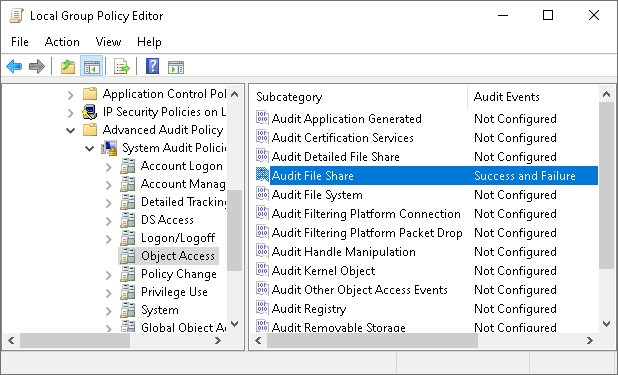
\includegraphics[width=\textwidth]{figures/audit-file-share.png}
  \caption[Screenshot of Local Group Policy Editor]{Screenshot of Local Group Policy Editor enabling file share auditing}
  \label{fig:audit-file-share}
\end{figure}

Since the events are so verbose and plentiful, they can also overlap quite a lot. For instance when a new account is created, the event "4720: A user account was created" is created, as well as the events "4722: A user account was enabled.", "4724: An attempt was made to reset an account's password" and "4738: A user account was changed". This is shown in \cref{fig:create-user-events}.

\begin{figure}[htbp]  % order of priority: h here, t top, b bottom, p page
  \centering
  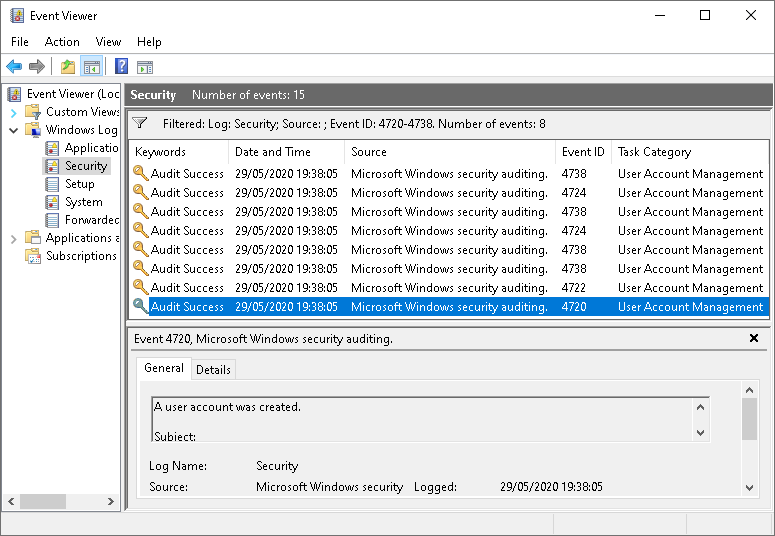
\includegraphics[width=\textwidth]{figures/create-user-events.png}
  \caption[Screenshot of events related to user creation]{Screenshot of events related to user creation}
  \label{fig:create-user-events}
\end{figure}

In enterprise networks that utilize Active Directory for managing multiple hosts, these type of \acrshort{gpo} settings can be configured centrally and applied to relevant machines. The above-mentioned file share events would for instance be interesting to enable for file servers, but not for other servers or client machines. If the enterprise uses some sort of central log collection, it is therefore necessary to configure and tune which events are saved, as that will affect how many events are sent over the wire and stored centrally.

When it comes to forwarding events and storing them, Windows Event logs are not stored in plain text on the system, but in a proprietary binary format as explained by \textcite{Schuster_2007}. To access the events programmatically, one have to go through the Windows Event Log \acrfull{api}\cite{Windows_event_log_api}. From the \acrshort{api} it is possible to access the raw \acrshort{xml} of the events. It is also possible to view the events in the built-in Event Viewer as seen in \cref{fig:event-viewer}. This is a program that allows for searching, filtering and viewing events. Each event contains a lot of information, and it is possible to view more details about each event as seen in \cref{fig:event-properties}.

\begin{figure}[htbp]  % order of priority: h here, t top, b bottom, p page
  \centering
  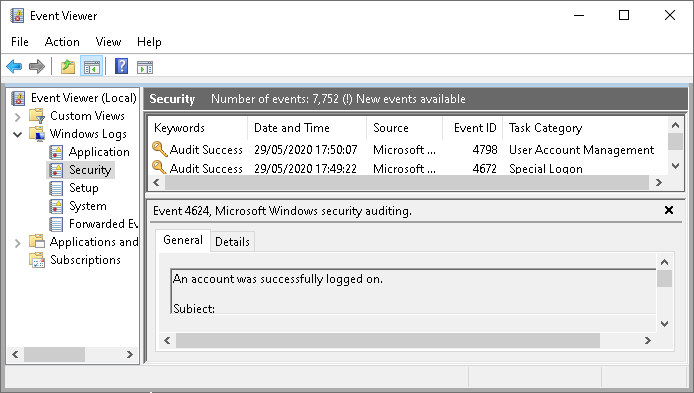
\includegraphics[width=\textwidth]{figures/event-viewer.png}
  \caption[Screenshot of Event Viewer]{Screenshot of Event Viewer}
  \label{fig:event-viewer}
\end{figure}

\begin{figure}[htbp]  % order of priority: h here, t top, b bottom, p page
  \centering
  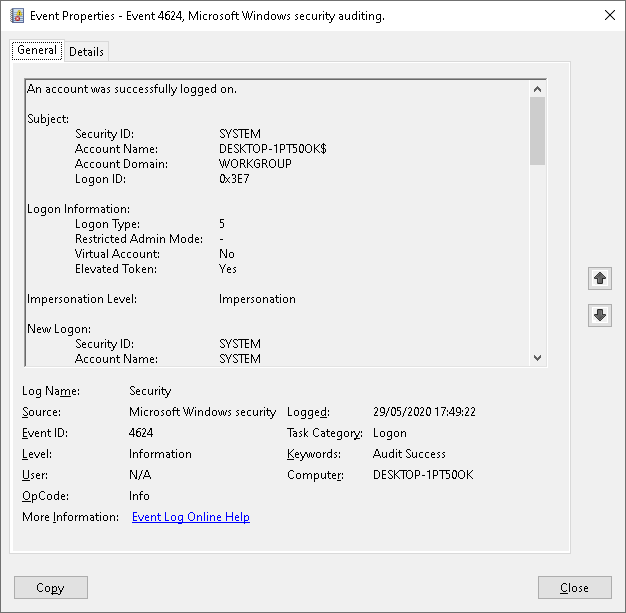
\includegraphics[width=\textwidth]{figures/event-properties.png}
  \caption[Screenshot of Event Properties]{Screenshot of Event Properties}
  \label{fig:event-properties}
\end{figure}

In enterprises, Windows Event Logs are usually sent to a centralized location for storage and analysis, either using the built-in option called Windows Event Forwarding\cite{windows_event_forwarding_docs} or using custom agents like Splunk Universal Forwarder\cite{Splunk_monitor_windows_event_log_data}, \textcite{Winlogbeat} or \textcite{nxlog_collecting_event_log_data} to name a few.

\subsubsection{Sysmon}
\acrfull{sysmon}\cite{Sysmon} is an extension to the stock Windows Event Logs that allows for a more powerful customization of what events go into the event log. Using a kernel driver, Sysmon is able to add support for a wider variety of interesting events. The table \ref{tab:sysmoneventtypes} is a list of each event type that Sysmon can generate.
Sysmon events do not replace those of regular Windows events, but creates events that contain detailed information about process creations, network connections, and changes to file creation time which can be used to help identify malicious or anomalous activity and understand how intruders and malware operate on your network.

For our experiments in this thesis, we will focus our attention towards the \acrshort{sysmon} process creation event (event ID 1). This event contains all the information necessary to detect which processes ran on a system, what its parent process was, what the command line arguments passed to the process was, and so forth.

\begin{table}[htbp]
\begin{tabular}{l|l}
ID & Description \\ \hline
1 & Process creation \\
2 & A process changed a file creation time \\
3 & Network connection \\
4 & Sysmon service state changed \\
5 & Process terminated \\
6 & Driver loaded \\
7 & Image loaded \\
8 & CreateRemoteThread \\
9 & RawAccessRead \\
10 & ProcessAccess \\
11 & FileCreate \\
12 & RegistryEvent (Object create and delete) \\
13 & RegistryEvent (Value Set) \\
14 & RegistryEvent (Key and Value Rename) \\
15 & FileCreateStreamHash \\
17 & PipeEvent (Pipe Created) \\
18 & PipeEvent (Pipe Connected) \\
19 & WmiEvent (WmiEventFilter activity detected) \\
20 & WmiEvent (WmiEventConsumer activity detected) \\
21 & WmiEvent (WmiEventConsumerToFilter activity detected) \\
22 & DNSEvent (DNS query) \\
255 & Error
\end{tabular}
\caption{List of Sysmon event types}
\label{tab:sysmoneventtypes}
\end{table}



\section{Event correlation}

As stated in \cref{sec:event-logs}, a event is something that happens at a point in time. Event correlation is a statistical relationship between random events that are not necessarily expressed by a rigorous functional relationship as stated by \textcite{Prokhorov_correlation_in_statistics}. This means that the relationship between two events is based on the fact that the conditional probability of one of the events occurring, given the occurrence of another event, is different from the unconditional probability. There exists numerous ways to determine the dependency between two events, like Pearson coefficient according to \textcite{PearsonC62:online}, Spearman's rank correlation coefficient as illustrated by \textcite{Spearman38:online}, Kendall rank correlation coefficient as described in \textcite{Kendallc32:online}, Goodman and Kruskal's gamma by \textcite{Goodman_1954} just to name a few.

Event correlation is usually applied when we want to create a higher level of understanding, based on the information found in the events. By correlating events, we can gather up smaller events that in and of them self are not worthy an alarm, and create an over-arching alarm that encompasses the smaller events. Event correlation can be used for a wide range of cases, like root-cause analysis, fault detection and future prediction and its usage can be found in areas such as market and stock trends, fraud detection, system log analysis, network management and fault analysis, medical diagnosis and treatment, et cetera. In the information security sphere, correlation can be used for things like detecting patterns of \acrfull{ddos} attacks as shown by \textcite{wei_2013} and identifying subsets of data attributes for intrusion detection as outlined by \textcite{Jiang_2004} and for detection of attacks based on the relationships between network events as shown in \textcite{kruegel_2004}.

Event correlation is a broad topic, and a complete overview is outside the scope of this thesis. The following sections will highlight some of the more popular event correlation methods, and particularly rule-based event correlation which will be the main focus for our thesis with regard to event correlation techniques. 

\iffalse
Many modern SIEM systems use a rule-based correlation \textcite{hanemann_2008} \textcite{limmer_2008}. It is based on a fixed correlation of events under certain conditions that may contain logical operations on data, their properties and calculated indicators. The main advantage of this method is ease of implementation. Its main drawbacks are as follows: the complexity and long time for computing the rules by the security administrator; its efficiency directly depends on the skills of administrator; and the system that uses such method is not able to detect the incidents if such rules were not initially specified for them.
There are also
methods based on templates (scenarios) \textcite{hanemann_2008}, graphs \textcite{ghorbani_2009} \textcite{xu_2006}, finite state machines \textcite{hasan_1999} \textcite{xu_2006}, similarity \textcite{gurer_1996} \textcite{zurutuza_2004}
and others, but they can also be expressed in the form of rules.
Currently, the methods that should eliminate these disadvantages are being
developed.

They are based on the intelligent data analysis. It refers to self-learning approaches such as Bayesian networks \textcite{bursztein2009using} \textcite{dantu2009network} \textcite{fedorchenko2017correlation}, immune networks \textcite{tiffany2002survey} \textcite{xu_2006}, artificial neural networks \textcite{elshoush2011alert} \textcite{kou2012evaluation} and others. For example, in \textcite{Jiang_2004} a probabilistic event correlation model for network attack detection based on spatial-temporal analysis is proposed. Here event spaces are linked in a chain of
sequences, and a concrete state from the set of states corresponds to each space at
the current moment. The resulting chain sequences are used to calculate the probability of a specific attack scenario. \textcite{davis2017resident} use the application behavior
model to identify illegitimate and abnormal activity. The initial data for constructing
the model are events that reflect the system calls of all possible applications. Based
on the initial information, a normal behavior profile is formed by processing a
multi-graph where each vertex is an event.
The advantage of these approaches is in the possibility of an independent
(unconditional) event correlation with minimization of manual settings. Their disadvantages are the complexity of learning model building, additional requirements
to the adequacy and quality of the models, and to the completeness of original
training data.
\fi

\iffalse
\subsection{Scenario-based Correlation}
https://dl.acm.org/doi/pdf/10.1145/1501434.1501479
\subsection{Statistical Correlation}
\subsection{Temporal Correlation}
\fi

\subsection{Finite State Machines}
% What are finite state machines?
A finite-state machine, a system is abstracted into mathematical model which can have exactly one of a finite number of states at a time. A finite-state machine has a fixed set of possible states, a set of inputs that change the state, and a set of possible outputs as described by \textcite{keller_2001}.
The next state of a finite-state machine is based on the current state that the machine is in, and the input that change the state.
There are generally considered to be two kinds of finite-state machines, deterministic finite-state machines and non-deterministic finite-state machines. In a deterministic finite-state machine, every state has only one transition per input, as opposed to the non-deterministic state machine, where an input can lead to none, one or many transitions for a given state. Since the deterministic finite-state machine is a more strict version of the non-deterministic finite-state machine, that leads to that by definition, a deterministic finite-state machine is also a non-deterministic finite-state machine.
For example, assuming that we have the following three events in order:
\begin{enumerate}
    \item the process '$word.exe$' started
    \item the process '$googlechrome.exe$' started
    \item The process '$powershell.exe$' started
\end{enumerate}
If we want to trigger an alert when we see the $word.exe$ process is created, and then the $powershell.exe$ process afterwards, we can design a simple non-deterministic state machine like the one in Figure \ref{fig:finite-state-machine}. When applying the above-mentioned events to this finite state-machine, event number one will move our state from $s_0$ to $s_1$. Event number two will not do any transitions and change the state (one of the benefits of using a non-deterministic state machine). When event number three occurs, the state machine transitions from $s_1$ to $s_2$, and our accepting state is reached, which fulfills the state machine and we can create an alarm.
\begin{figure}[ht]
\centering
\begin{tikzpicture}[->,>=stealth',shorten >=1pt,auto,node distance=4cm,
                    thick,main node/.style={circle,draw,font=\sffamily\Large\bfseries}]
  \node[initial,state] (p1) {$s_0$};
  \node[state] (p2) [right of=p1] {$s_1$};
  \node[state,accepting] (p3) [right of=p2] {$s_2$};

  \path[every node/.style={font=\sffamily\small}]
    (p1)
        edge node {'word.exe' started} (p2)
    (p2)
        edge node {'powershell.exe' started} (p3)
    ;
\end{tikzpicture}
\caption{Example of non-deterministic finite-state machine}
\label{fig:finite-state-machine}
\end{figure}
One of the benefits of the finite-state model is that it is possible to specify if the order of the events are important or not. If the event order is not of interested, a finite-state machine as shown in Figure \ref{fig:finite-state-machine-2} can represent the same case as seen in Figure \ref{fig:finite-state-machine}.
\begin{figure}[ht]
\centering
\begin{tikzpicture}[->,>=stealth',shorten >=1pt,auto,node distance=1.5cm,
                    thick,main node/.style={circle,draw,font=\sffamily\Large\bfseries}]
  \node[initial,state] (s0) {$s_0$};
  \node[] (middle) [right of=s0] {};
  \node[state] (s1) [above of=middle] {$s_1$};
  \node[state] (s2) [below of=middle] {$s_2$};
  \node[state,accepting] (s3) [right of=middle] {$s_3$};

  \path[every node/.style={font=\sffamily\small}]
    (s0)
        edge node {'word.exe' started} (s1)
        edge node [swap] {'powershell.exe' started} (s2)
    (s1)
        edge node {'powershell.exe' started} (s3)
    (s2)
        edge node [swap] {'word.exe' started} (s3)
    ;
\end{tikzpicture}
\caption{Example of non-deterministic finite-state machine}
\label{fig:finite-state-machine-2}
\end{figure}

An approach to use finite-state machines for event correlation has been shown by \textcite{Bouloutas_1992}. The authors use observed events that are generated by the monitored process to feed into the modelled finite-state machine that represent the monitored process. If an event arrives that leads to an invalid state in the model, an error is produced.

One of the main drawback with the finite-state machine is the missing notion of time. As shown in Figure \ref{fig:finite-state-machine-2} we can take into account order of events, but a finite-state machine does not separate on the time difference between events that are streamed into the model.

\subsection{Rule-based Event Correlation}
\label{sub:rule-based-event-correlation}
Rule-based event correlation software is historically known as a expert system. Expert systems is defined by \textcite{cronk_1988} as a "problem-solving software that embodies specialized knowledge in a narrow task domain to do work usually performed by a trained, skilled human.". According to \textcite{cronk_1988}, expert systems are organized around three levels; data, control and knowledge. As shown in \cref{fig:rule-based-expert-system}, the data level is the working memory of the expert system that contains the events that are being processed. Then the knowledge level is the rule repository that contains the domain-specific expert knowledge. Finally we have the control level which consist of the inference engine that determines how to apply the rules from the knowledge base against the working memory.

\begin{figure}[htbp]
\centering
%\tikzstyle{startstop} = [rectangle, rounded corners, minimum width=3cm, minimum height=1cm,text centered, draw=black, fill=red!30]
\begin{tikzpicture}[->,>=stealth',shorten >=1pt,auto,node distance=6cm,
                    thick,main node/.style={circle,draw,font=\sffamily\Large\bfseries},
                    problemm/.style={circle, text centered, draw=black, fill=red!30},
                    stepp/.style={rectangle, minimum width=7cm, minimum height=1cm,text centered, draw=black, fill=orange!30},
                    libraryy/.style={rectangle, rounded corners, minimum width=3cm, minimum height=1cm,text centered, draw=black, fill=green!30}]
  \node (workingmemory) [stepp] {Working Memory};
  \node (inferenceengine) [stepp, below of=workingmemory] {Inference Engine};
  \node (knowledgebase) [stepp, below of=inferenceengine] {Knowledge Base};
  
  \path[every node/.style={font=\sffamily\small}]
    (workingmemory)
        edge[bend left, text width=2.0cm, align=center] node {Remove data elements} (inferenceengine)
    (inferenceengine)
        edge[bend left, text width=2.0cm, align=center] node {Create new data elements} (workingmemory)
        edge[text width=1.6cm, align=center] node[anchor=center,fill=white] {Modify attributes of data elements} (workingmemory)
        edge[bend right, text width=2.0cm, align=center, swap] node {Match potential rule} (knowledgebase)
    (knowledgebase)
        edge[text width=1.6cm, align=center] node[anchor=center,fill=white] {Select "best" rule} (inferenceengine)
        edge[bend right, text width=2.0cm, align=center, swap] node {Invoke action} (inferenceengine)
        
    ;
\end{tikzpicture}
\caption{Model of rule-based expert systems}
\label{fig:rule-based-expert-system}
\end{figure}

Traditionally, creating the rules that goes into a knowledge base is defined as two-fold; first you have the subject-matter expert which has the expertise and knowledge about which events you are interested in creating correlations against, and secondly the knowledge engineer which is familiar with how the expert system works and how the rules has to be written to be understood by the system.
In more modern settings, usually the subject-matter expert and the knowledge engineer is the same person. This person has both the knowledge of which events are of interest, and the capability to implement, monitor and tune the rules necessary to detect the events that are of interest.

The value of a rule-based approach is that the rules in the knowledge base can be written with a close similarity to the human language. For example if we want to write a rule for the occurrence of two different events X and Y, it could be spelled out like "\textit{\textbf{IF} event X \textbf{AND} event Y \textbf{THEN} doAction}". This also makes it easier to deduce how and why an alert was triggered. We will take a further look at different rules that can be utilized with rule-based event correlation in \cref{sec:rules}.

In larger production environments, it is also important that the rules are specific enough, so that they do not generate too many alarms.
There can be multiple reasons that a rule will trigger too many times. If the subject-matter expert is not specific enough when defining which conditions are to be added to the rule, or there can be a lack of proper events to analyze, such that to catch the behaviour that the subject-matter expert wants to detect, the knowledge engineer will have to write a more generic rule than wanted. Regardless, the knowledge engineer will have to tune the rule such that it will not flood the analysts with new alerts. Commonly such rules are ran in a test system with production input such that the knowledge engineer can collect metrics on how often the rules trigger alerts before adding the rule to production.

One of the main drawbacks, and probably the biggest reason for other types of event correlation is the lack of learning or adaptability, which menas that the same correlation will be made for every similar case every time as stated by \textcite{meira1997model}. Networks may differ, so it is not given that a rule that fits into one network, can automatically be used in another. As outlined by \textcite{lewis_1993}, rule-based correlation tend to fail when presented with new or unexpected situations. In addition, creating new rules, maintaining old rules and adapting the rules in the knowledge base can be time-consuming.
Regardless of these drawbacks, we see a common trend that rule-based systems are the most common when it comes to network-based monitoring (see \textcite{Suricata49:online}, \textcite{SnortNet49:online}) as well as for log data in \acrshort{siem}s like \textcite{Splunk}, \textcite{OSSEC} and \textcite{OSSIM}.

There exists several different types of software that makes it possible to correlate events in real-time based on log data. From more simple projects like \textcite{swatchdog}, LogSurfer \cite{thompson_2017} and \acrshort{sec} \cite{SEC}, to more complex projects with multiple moving parts like \textcite{Prelude:online}, \textcite{OSSEC}, \textcite{Wazuh:online}, \textcite{ApacheMe75:online}, \textcite{MozDef}, \textcite{OpenNMS}, \textcite{OSSIM}.

Throughout most of the literature regarding event correlation of log data, \acrfull{sec} \cite{SEC} has stuck out as one of the most popular software for doing event correlation on log data, as seen in \textcite{kont2017frankenstack}, \textcite{farshchi2018anomaly} and \textcite{vaarandi2003data} just to name a few. I will address \acrshort{sec} further under \cref{sec:SEC}.

\subsection{Case-based Reasoning}

In case-based reasoning, a previously experienced problem and its solution is called a case. Case-based reasoning is based on the assumption that we can find a solution for a new problem by finding past cases that are similar, and then reusing the solution to solve the new problem. The reasoning is then further enforced by adding the problem and the solution to the case library for future use as described by \textcite{aamodt_1994}.
As stated by \textcite{slade_1991}, case-based reasoning is similar to how humans approach new problems by assimilating past experiences and adapting them to new situations.

Figure \ref{fig:case-based-reasoning-cycle} describes the cycle used in case-based reasoning from a high-level perspective.
Under each step in the cycle there are multiple tasks that may be necessary to conduct before continuing on with the cycle. For instance, the "Retrieve" step might need to identify which features of the problem to search the Case Library for.
\begin{figure}[ht]
\centering
%\tikzstyle{startstop} = [rectangle, rounded corners, minimum width=3cm, minimum height=1cm,text centered, draw=black, fill=red!30]
\begin{tikzpicture}[->,>=stealth',shorten >=1pt,auto,node distance=2cm,
                    thick,main node/.style={circle,draw,font=\sffamily\Large\bfseries},
                    problemm/.style={circle, text centered, draw=black, fill=red!30},
                    stepp/.style={rectangle, minimum width=3cm, minimum height=1cm,text centered, draw=black, fill=orange!30},
                    libraryy/.style={rectangle, rounded corners, minimum width=3cm, minimum height=1cm,text centered, draw=black, fill=green!30}]
  \node (Problem) [problemm] {Problem};
  \node (Retrieve) [stepp, below of=Problem] {Retrieve};
  \node (Reuse) [stepp, below of=Retrieve] {Reuse};
  \node (Revise) [stepp, below of=Reuse] {Revise};
  \node (Retain) [stepp, right of=Revise, xshift=3cm] {Retain};
  \node (CaseLibrary) [libraryy, right of=Retrieve, xshift=3cm] {Case Library};
  
  \path[every node/.style={font=\sffamily\small}]
    (Problem)
        edge node {} (Retrieve)
    (Retrieve)
        edge node {} (Reuse)
    (Reuse)
        edge node {Copy or Adapt} (Revise)
    (Revise)
        edge node {Evaluate} (Retain)
    (Retain)
        edge node {} (CaseLibrary)
    (CaseLibrary)
        edge node {} (Retrieve)
    ;
\end{tikzpicture}
\caption{Case-based reasoning cycle}
\label{fig:case-based-reasoning-cycle}
\end{figure}

A example where this might be useful is in a Security Operations Center (SOC). A SOC receives a high number of alerts that have to be handled by an analyst to analyse and propose a response to the alert. The response can vary from simply suppressing the alert as a false-positive, sending an e-mail to the client to alert them, or escalating the alarm to the Incident Response team. Case-based reasoning can then be applied to new alerts by first retrieving the most similar alerts previously handled. The information stored in the previous case can then be used to handle the analysis or solution to an alert. The analyst will then revise the proposed solution, and retain the parts that might be useful for resolving similar future alerts. This follows the case-based reasoning cycle proposed in \citetitle{aamodt_1994} by \textcite{aamodt_1994}.

The retrieval step is difficult because we need to find similar cases that offer solutions that are relevant. Cases may contain attributes that are irrelevant, which might not be clear to the automated retrieval process.
An example of this could be the following: Consider that we receive an alert that a malicious file has been detected on a system. We get the IP, hostname, filename and hash of the file as part of the alert. The analyst decides that the file is benign through analysis. This is then stored as a case. If we then receive another similar alert containing yet again an IP, hostname, filename and hash of the file. The filename in this new alert is identical to the one we received earlier, but the hash is different. Using this data, the case-based reasoning engine should not propose a solution based the fact that the filenames are identical, since the file hashes are different, suggesting that the files are not the same.
To solve this, both the work by \textcite{lewis_1993} and \textcite{davies_1987} propose creating "determination rules" or "determinators" that are either compound attributes or a pointer to which attributes to look at in the case.
Additionally, adaptation of the old solutions to the new problem is a difficult task. While manual specification of the solution in the "Revise" step is possible and somewhat required, too much emphasis on manual intervention or adjustments will defeat the purpose of case-based reasoning. This is why according to \textcite{leake_1996} many case-based reasoning systems have adapted the cycle from Retrieve-Reuse-Revise-Retain to a much shorter Retrieve-Propose cycle that completely eliminates the adaptation.

In the paper \citetitle{schwartz_2002}, the authors \textcite{schwartz_2002} used the intrusion detection system Snort as a basis for a new case-based reasoning IDS that uses the Snort rule base as a case library. Snort rules may in general be too specific and fail to detect certain kind of intrusions, but with the case-based reasoning approach, the retrieval step in the cycle will take care of this by finding cases (rules) that are applicable to the network packet even though the vanilla rule would not create an alert on that packet.
\textcite{Kapetanakis_2014} argue that with the digital traces left by an attacker, it is possible to build a profile for that attacker which can be used to assist in future attacks to identify which attacker is attacking. In the paper written by \textcite{han_2016}, the authors implemented a system called "WHAP" which uses case-based reasoning to compare cyber attacks against websites. WHAP builds on a large database of website defacements, which are custom webpages left on the victim server by the attacker to claim credit for a website hack. The system is then able to take new hacked websites as input, and output similar previous cases where it is likely that the website has been hacked by the same attacker. This can be useful for attribution and forensic investigations.

\subsection{Model-based Reasoning}
Model-based reasoning is a expert system where the target is to create a model that can be used to predict the outcome of input event or faults in the system. The idea of modelling the structure and behavior of a system has its roots in the work done by \textcite{davies_1987} where they explore the use of such models in troubleshooting digital electronics.  There are no fixed way for how a system can or should be modelled. The model itself can be created as a logical formalization using pure mathematics, or as a simulated system using for example a game engine. As \textcite{Dodig-Crnkovic2017} highlight in their paper \citetitle{Dodig-Crnkovic2017}, there is an increased interest in automating the creation of the model of a system. This is based on the fact that creating and keeping a model consistent with the system it is supposed to model, is hard.
\textcite{jakobson_1993} discuss model-based reasoning for alarm correlation for fault management in telecommunications networks in their paper \citetitle{jakobson_1993}.


\iffalse


The managed system is modeled
with respect to its event emission behavior (event model). The programmed knowledge somehow
defines events to be related under some temporal or sequential constraints

A description of the 


structure, the topology, connectivity of components
behaviour description,
a set of principles to guide the troubleshooting \textcite{davies_1987}

\fi

In \citetitle{poll_2003} written by \textcite{poll_2003}, a figure similar to \ref{fig:model-based-reasoning-example} is shown. It outlines the process for checking if a modelled system is consistent with the real world system it is supposed to replicate.

\begin{figure}[ht]
\centering
\begin{tikzpicture}[->,>=stealth',shorten >=1pt,auto,node distance=2cm,thick
                    ]
  \node (PhysicalSystem) [xshift=-1cm] {Physical system};
  \node (Model) [xshift=1cm, right of=PhysicalSystem] {Model of system};
  \path (PhysicalSystem) -- (Model) coordinate[midway] (aux);
  
  \node (Actions) [below of= aux] {Actions};
  
  \node (Observed) [below of= Actions,xshift=-2cm] {Observed behavior};
  \node (Predicted) [below of= Actions,xshift=2cm] {Predicted behavior};
  \path (Observed) -- (Predicted) coordinate[midway] (aux2);
  
  \node (Discrepancy) [below of= aux2] {Discrepancy?};
  
  \node (no) [below of= Discrepancy,xshift=-2cm,text width=3.5cm] {Model is consistent with system};
  \node (yes) [below of= Discrepancy,xshift=2cm,text width=3.5cm] {Search over model\\to explain discrepancy};
  
  \path[every node/.style={font=\sffamily\small}]
    (PhysicalSystem)
        edge node {} (Actions)
    (Model)
        edge node {} (Actions)
    (Actions)
        edge node {} (Observed)
        edge node {} (Predicted)
    (Observed)
        edge node {} (Discrepancy)
    (Predicted)
        edge node {} (Discrepancy)
    (Discrepancy)
        edge node [swap] {No} (no)
        edge node {Yes} (yes)
    ;
\end{tikzpicture}
\caption{Illustration of model-based reasoning}
\label{fig:model-based-reasoning-example}
\end{figure}
As stated by \textcite{sethi_2001}, one of the primary drawbacks of model-based reasoning is the requirement to have a well structured system to model and to keep that model updated. Systems that contain fluctuating objects like for example computer networks or network services are not trivial to represent in a formal model. More applicable areas might include hardware diagnostics like shown in the work by \textcite{davies_1987}, or other areas where it is possible to model a more static target system, like for example automobile diagnostics. Finally, in \citetitle{Venkatasubramanian_2003} by \textcite{Venkatasubramanian_2003}, they discuss that various implementations of model-based reasoning is quite computational complex, depending on number of objects in the model and their various inputs and outputs.

\subsection{Codebook-based Event Correlation}
\label{sub:codebook-based-event-correlation}

\begin{figure}[ht]
\centering
\begin{tikzpicture}[->,>=stealth',shorten >=1pt,auto,node distance=3cm,
                    thick,main node/.style={circle,draw,font=\sffamily\Large\bfseries}]
  \node[main node] (p1) {$p^1$};
  \node[main node] (p2) [right of=p1] {$p^2$};
  \node[main node] (p3) [right of=p2] {$p^3$};
  \node[main node] (e1) [below left of=p1] {$e^1$};
  \node[main node] (e2) [right of=e1] {$e^2$};
  \node[main node] (e3) [right of=e2] {$e^3$};
  \node[main node] (e4) [right of=e3] {$e^4$};

  \path[every node/.style={font=\sffamily\small}]
    (p1)
        edge node {} (e1)
        edge node {} (e2)
        edge node {} (e3)
    (p2)
        edge node {} (e2)
        edge node {} (e3)
        edge node {} (e4)
    (p3)
        edge node {} (e1)
        edge node {} (e2)
        edge node {} (e4)
    ;
\end{tikzpicture}
\caption{Example causality graph used for codebook-based event correlation}
\label{fig:causality-graph-codebook}
\end{figure}

\textcite{yemini_1996} propose that the events caused by problems can be modelled as seen in figure \ref{fig:causality-graph-codebook} where the directed edges of the graph describe the causality of an event. $p^x$ denotes a problem, and $e^x$ denotes an event. To utilize the codebook, each problem node in the graph is converted into a binary vector that can be used to describe its relation to the events on the graph. This is known as a "code". The binary vector contains bits that corresponds to each event in the graph. If a bit is set to a $1$, it indicates that the given problem causes the event that the bit corresponds to. A bit of $0$ indicates that it does not cause the event. These codes then go into the codebook. If we convert the graph in figure \ref{fig:causality-graph-codebook} into a codebook, it will look like table \ref{tab:correlation-matrix}. The graph and codebook needs to be sufficiently large to be able to identify all the problems. If the codebook is too small, it may omit events that are of interest to us. If the codebook is too large, it may contain events that are unnecessarily redundant. One way to approach the problem with codebooks that are too large, is to do what \textcite{yemini_1996} calls "codebook reduction". Codebook reduction is the process of removing events that are "universal" for all problems. In the figure \ref{fig:causality-graph-codebook} and the corresponding table \ref{tab:correlation-matrix} we can see that event $e^2$ is a common event for all the problems. Because of this redundancy, it can be remove to simplify the codebook as show in table \ref{tab:correlation-matrix-reduced}. Further work has been done to enhance the efficiency of the codebook. \textcite{gupta_1999} proposes a two step preprocessing algorithm that ensures mathematical provable codebooks and eliminates events that are unable to distinguish between problems.

When new events occur, the events are converted into a new binary vector. This vector is then compared with the codes in the codebook, and the code that is the most similar is chosen as a means to identify the problem. A simple approach for comparing the binary vectors could be a 1-to-1 comparison to see if the new binary vector exactly matches any of the codes in the codebook, but \textcite{yemini_1996} propose to instead use Hamming distance to calculate the closest match. Using Hamming distance has several benefits, first of all it increases the tolerance for noise or lost events, secondly instead of choosing a single best candidate problem, we can defined a radius that will give us a codebook subset containing possible codes within the given Hamming distance radius.
Because of the novel preprocessing down to binary vectors, codebook-based correlation is faster than other rule-based event correlation techniques. One of the more time-consuming tasks with regard to codebook-based event correlation is the creation of the problems and their mapping to symptom events. The most likely way to produce these codebooks will be as an expert system where a person with deep knowledge about the events in the system are able to map symptoms to problems. In addition, the process of selecting which events might be symptoms of a problem is similar to feature selection in the machine learning landscape. Feature selection is the process of selecting a subset of features that can be used in model construction, which is similar to how the codebook is generated.

One of the biggest limitations regarding codebook-based event correlation is that there is no built-in way to handle time. When a problem has been identified based on a number of symptoms, there is no time window applied, and there is no notion of event order. Furthermore the events do not contain any properties, and would require significant extending to take into account e.g. source hostname, username.

\begin{table}[ht]
\centering
\begin{tabular}{l|llll}
 & $e^1$ & $e^2$ & $e^3$ & $e^4$ \\ \hline
$p^1$ & 1 & 1 & 1 & 0 \\
$p^2$ & 0 & 1 & 1 & 1 \\
$p^3$ & 1 & 1 & 0 & 1
\end{tabular}
\caption{Codebook correlation matrix}
\label{tab:correlation-matrix}
\end{table}

\begin{table}[ht]
\centering
\begin{tabular}{l|lll}
 & $e^1$ & $e^3$ & $e^4$ \\ \hline
$p^1$ & 1 & 1 & 0 \\
$p^2$ & 0 & 1 & 1 \\
$p^3$ & 1 & 0 & 1
\end{tabular}
\caption{Reduced codebook correlation matrix}
\label{tab:correlation-matrix-reduced}
\end{table}

\subsection{Dependency Graphs}


\begin{figure}[ht]
\centering
\begin{tikzpicture}[->,>=stealth',shorten >=1pt,auto,node distance=3cm,
                    thick,main node/.style={circle,draw,font=\sffamily\Large\bfseries}]
  \node[main node] (a) {$a$};
  \node[main node,fill=blue] (b) [right of=a] {$b$};
  \node[main node,fill=blue] (c) [right of=b] {$c$};
  \node[main node,fill=blue] (d) [below left of=a] {$d$};
  \node[main node] (e) [right of=d] {$e$};
  \node[main node] (f) [right of=e] {$f$};
  \node[main node] (g) [right of=f] {$g$};
  \node[main node] (h) [below left of=d] {$h$};
  \node[main node,fill=red] (i) [right of=h] {$i$};
  \node[main node] (j) [right of=i] {$j$};
  \node[main node] (k) [right of=j] {$k$};
  \node[main node] (l) [right of=k] {$l$};

  \path[every node/.style={font=\sffamily\small}]
    (a)
        edge node {} (e)
    (b)
        edge node {} (e)
    (c)
        edge node {} (f)
    (d)
        edge node {} (h)
        edge node {} (i)
    (e)
        edge node {} (j)
    (f)
        edge node {} (j)
        edge node {} (k)
    (g)
        edge node {} (k)
        edge node {} (l)
    (j)
        edge node {} (i)
    ;
\end{tikzpicture}
\caption{Example dependency graph}
\label{fig:dependency-graph}
\end{figure}

Similar to the dependency graph used in \ref{sub:codebook-based-event-correlation}, \textcite{Gruschke_1998} suggests that a dependency graph can contain enough information to be used for event correlation, while also being simple to automatically generate. The dependency graph is a directed graph that maps the relationship managed objects. These objects can be hosts in a network, dependencies between software dependencies, and so forth.
In figure \ref{fig:dependency-graph} we have mapped a series of objects as an example. Events are mapped to their corresponding object in the graph (colored in blue, object b, c and d). Then we walk the graph from those objects. As explained by \textcite{Gruschke_1998}, when we optimally find one object node that are common for all the given events, we have most likely found the responsible node. In the example this is marked as red, object i.
\textcite{Gruschke_1998} further outlines that the quality of the root-cause detection can be measured by the depth and length we need to walk the graph at. Objects that are further away from the initial object are less likely to be the root cause, and vica versa.
One of the main drawbacks of dependency-graph-based correlation is the fact that it does not handle multiple, non-related problems very well. \textcite{Gruschke_1998} assumes that only one problem occurs at a time. If multiple problems occur that are not related or affect each other, finding the root-case may prove to be impossible, or select the wrong root-cause object.
Assumes the events are for a single fault. Meaning it will not be able to handle detecting multiple failing nodes.
As with the codebook-based event correlation we discussed in \ref{sub:codebook-based-event-correlation}, dependency graphs also lack the notion of time. Additionally the dependency graph is not taking advantage of attributes on the nodes to further enhance the graph.

\subsection{Bayesian Network-based Event Correlation}

Bayesian networks are one of the most widely used graphical models for representing and reasoning about the probabilistic causal relationships between variables as explained in \textcite{Kavousi_2014}. Bayesian networks are usually represented by directed acyclic graphs. Directed acyclic graphs are finite directed graphs that contain no direct cycles. This means that there is no way to start from a given node, and via the directed edges return back to the same node. Each node in the network represents a variable of interest and the edges describe the relations between these variables.
The Bayesian network is split up into two parts. First there is the graphical model of the network which shows the nodes and the edges that connect them. Secondly, there is the conditional probability tables associated with each node. The table consist of the probabilities that a node is in a given state given the state of its parent nodes.



Both the research done by \textcite{Kavousi_2014} and \textcite{Qin_2004} utilize Bayesian networks to create "Bayesian attack graphs" (BAG) which are models that use Bayesian networks to depict the security attack scenarios in a system.

As a simple experiment using a Bayesian Network for detection, we have the directed acyclic graph as shown in Figure \ref{fig:simple-directed-acyclic-graph}. The nodes are a bit like the ones represented in Codebook-based correlation \ref{sub:codebook-based-event-correlation} where the nodes $B$ and $C$ represent two symptom events that are analyzed by the system, these can be events from an IDS, host machine logs, web logs, et cetera. The node $A$ represent a problem node and is not connected to any specific events. The purpose of this Bayesian network, is to answer the following question: What is the probability that, when we observe the two events $B$ and $C$, we have a problem $A$?

To calculate this, we first need the the conditional probability tables, which are given in Table \ref{tab:probabability-tables}.

\begin{figure}[ht]
\centering
\begin{tikzpicture}[->,>=stealth',shorten >=1pt,auto,node distance=1cm,
                    thick,main node/.style={circle,draw,font=\sffamily\Large\bfseries}]
  \node[main node] (a) {$A$};
  \node[main node] (b) [below of=a,xshift=-2cm] {$B$};
  \node[main node] (c) [below of=a,xshift=2cm] {$C$};

  \path[every node/.style={font=\sffamily\small}]
    (a)
        edge node {} (b)
        edge node {} (c)
    ;
\end{tikzpicture}
\caption{Simple example directed acyclic graph}
\label{fig:simple-directed-acyclic-graph}
\end{figure}

\begin{table}[ht]
\centering
\begin{tabular}{|l|l|}
\hline
$P(A = 0)$ & $P(A = 1)$ \\ \hline
$0.8$ & $0.2$ \\ \hline
\end{tabular}
\begin{tabular}{|l|l|l|}
\hline
$A$ & $P(B = 1|A)$ & $P(B = 0|A)$ \\ \hline
$1$ & $0.9$ & $0.1$ \\ \hline
$0$ & $0.05$ & $0.95$ \\ \hline
\end{tabular}
\centering
\begin{tabular}{|l|l|l|}
\hline
$A$ & $P(C = 1|A)$ & $P(C = 0|A)$ \\ \hline
$1$ & $0.95$ & $0.05$ \\ \hline
$0$ & $0.05$ & $0.95$ \\ \hline
\end{tabular}
\caption{Conditional probability tables}
\label{tab:probabability-tables}
\end{table}

We can then calculate the probability that $A$ has occurred, given that we have observed the events $B$ and $C$ by using Bayes' theorem.
\begin{align*}
    &P(A=1 | B=1, C=1)\\
    &=\frac{P(A=1)P(B=1,C=1|A=1)}{P(B=1,C=1)}\\
    &=\frac{P(A=1)P(B=1,A=1)P(C=1,A=1)}{P(A=1)P(B=1|A=1)P(C=1|A=1)+P(A=0)P(B=1|A=0)P(C=1|A=0)}\\
    &=\frac{0.2\cdot0.9\cdot0.95}{(0.2\cdot0.9\cdot0.95)+(0.8\cdot0.05\cdot0.05)}\\
    &\approx 0.9884
\end{align*}
In this case, we see that there is a 98.8\% chance that the problem/alert $A$ has happened, by observing the arrival of the two events $B$ and $C$.


\subsection{Neural Network Approaches}
Artificial Neural Networks are used in the field of Artificial Intelligence as a system that is inspired by the neural networks in biological brains as explained by \textcite{chen2019design}. These system often come in the form of highly interconnected, neuron-like processing units. As illustrated in \cref{fig:neural-network}, the circular node represents an artificial neuron and an arrow represents a connection from the output of one artificial neuron to the input of another.
These systems are meant to learn and perform tasks by ingesting training data, and creating their own decision model that will be applied when considering future cases.

\begin{figure}
    \centering
    \def\layersep{2cm}
\begin{tikzpicture}[
   shorten >=1pt,->,
   draw=black!50,
    node distance=\layersep,
    every pin edge/.style={<-,shorten <=1pt},
    neuron/.style={circle,fill=black!25,minimum size=17pt,inner sep=0pt},
    input neuron/.style={neuron, fill=green!50},
    output neuron/.style={neuron, fill=red!50},
    hidden neuron/.style={neuron, fill=blue!50},
    annot/.style={text width=4em, text centered}
]

    % Draw the input layer nodes
    \foreach \name / \y in {1,...,4}
    % This is the same as writing \foreach \name / \y in {1/1,2/2,3/3,4/4}
        \node[input neuron, pin=left:Input \#\y] (I-\name) at (0,-\y) {};

    % set number of hidden layers
    \newcommand\Nhidden{3}

    % Draw the hidden layer nodes
    \foreach \N in {1,...,\Nhidden} {
       \foreach \y in {1,...,5} {
          \path[yshift=0.5cm]
              node[hidden neuron] (H\N-\y) at (\N*\layersep,-\y cm) {};
           }
    \node[annot,above of=H\N-1, node distance=1cm] (hl\N) {Hidden layer \N};
    }

    % Draw the output layer node
    \node[output neuron,pin={[pin edge={->}]right:Output}, right of=H\Nhidden-3] (O) {};

    % Connect every node in the input layer with every node in the
    % hidden layer.
    \foreach \source in {1,...,4}
        \foreach \dest in {1,...,5}
            \path (I-\source) edge (H1-\dest);

    % connect all hidden stuff
    \foreach [remember=\N as \lastN (initially 1)] \N in {2,...,\Nhidden}
       \foreach \source in {1,...,5}
           \foreach \dest in {1,...,5}
               \path (H\lastN-\source) edge (H\N-\dest);

    % Connect every node in the hidden layer with the output layer
    \foreach \source in {1,...,5}
        \path (H\Nhidden-\source) edge (O);

    % Annotate the layers

    \node[annot,left of=hl1] {Input layer};
    \node[annot,right of=hl\Nhidden] {Output layer};
\end{tikzpicture}
    \caption{Example of neural network with three hidden layers}
    \label{fig:neural-network}
\end{figure}


The computation done in each node can vary from simple mathematical operations like a summation of all its inputs, or by using more complex operations like treshold values, temporal operation as explained by \textcite{lippmann1987introduction} or operations that involve the memory of a node as shown in \textcite{meira1997model}. To allow the network to learn, input weights are often dynamically adapted as stated by \textcite{lippmann1987introduction}. Which strategy is used for operation selection and input weighting depends on the application of the network, and multiple approaches exist for this.

As \textcite{pouget2003alert} stated in their paper \citetitle{pouget2003alert}, "Neural Networks seem not to be frequently applied in Alert Correlation tools.". The primary reason for this is that it is hard to get insight into how a neural network arrived at the output it produced. Regardless, there are several papers that use artificial intelligence and neural networks for event correlation. The authors of \citetitle{friedberg2015combating} \textcite{friedberg2015combating} automatically generated a system model with the ability to continuously evolve itself. The proposed approach was able to detect anomalies that are the consequence of realistic APT attacks. In the work by \textcite{lin2019detecting}, the authors used a distributed gradient boosting library to classify real-world malware programs with more than 99\% success-rate. Another approach is presented in \citetitle{wietgrefe1997using}, where the authors \textcite{wietgrefe1997using} used a neural network to correlate alarms in a cellular phone network.

One of the primary benefits of using neural networks is the ability the networks has to adapt either via training data, or in real time during processing of live event. As pointed out by \textcite{pouget2003alert}, the main drawback speaks to the fact that it is hard for an analyst to comprehend how a artificial neural network has concluded, which may affect the trust in the system.

\subsection{Hybrid approaches}
In additional to all the "pure" correlation techniques, there also exist various implementations that take a hybrid approach to event correlation by utilizing two or more techniques at the same time.
Some examples include the work done by \textcite{hanemann_2008} which combine rule-based event correlation and case-based reasoning, the authors of \citetitle{saad2012extracting}, \textcite{saad2012extracting} proposed a hybrid event correlation approach that used semantic analysis and a intrusion ontology to reconstruct attack scenarios. Furthermore, \textcite{ficco2013security} developed a hybrid, hierarchical event correlation approach for detecting complex attacks in cloud computing. Finally \textcite{Ludovic_2004} to proposed a fully functional\acrshort{ids} based on event and alert correlations by implementing a language driven signature based correlation that uses \acrshort{fsm} to implement the multi-pattern rule matching detection algorithm.

\section{Simple Event Correlator}
\label{sec:SEC}

As previously stated, throughout the relevant research done with regards to event correlation of system logs, \acrshort{sec} seems to be the most commonly referenced and used software. It is widely used and as \textcite{vaarandi2005tools} explains, has been deployed in several different sectors and industries (Finance, Telecom, IT security, Government, Retail, etc.). \acrshort{sec} has been utilized for several different purposes like fraud detection, insider-threat detection, system fault and availability and security events.

SEC is quite versatile, as it is agnostic to the type of log event that it receives. SEC uses rules that are using Perl-style regular expressions for matching events and extracting data from the event itself using sub-expressions. The extracted data can then be used to correlate between other matching events.

\iffalse
SEC reads lines from files, named pipes, or standard input, matches the lines with patterns (like regular expressions or Perl subroutines) for recognizing input events, and correlates events according to the rules in its configuration file(s). SEC can produce output by executing external programs (e.g., snmptrap or mail), by writing to files, by sending data to TCP and UDP based servers, by calling precompiled Perl subroutines, etc.
\fi

The rules used in \acrshort{sec} are heavily based on regular expressions, which makes it hard to understand, modify and write new rules. The argument for using regular expressions builds on the assumption that most system and network administrators are already familiar with the regular expression language as stated in \textcite{vaarandi2002sec}. Although that might be the case, complex regular expressions can be hard to comprehend, and the output of the regular expression also requires detailed knowledge of what the input event looks like. The rule format of \acrshort{sec} will be further explained under \cref{sub:sec-rule-format}.
In addition to this, there are few open source rules and rule-sets with a focus on security, which means that the analyst generally has to start from scratch writing their own rules.

Perhaps the biggest drawback of \acrshort{sec} is that \acrshort{sec} bases its correlation time on when the event was read from the input file. It does not take into account any timestamps that may be in the logs.
If logs are ingested from multiple systems (like a enterprise environment) the logs could be delayed for multiple reasons, or if \acrshort{sec} is unable to ingest the log events fast enough (either because of I/O delays or a huge amount of logs), the timestamp of the logs will be different from when the log event was \textit{actually} produced. The consequences of this could be severe, as events that should be correlated together in a given timeframe might drift away from each-other and not be correlated at all.

Scaling is possible, but a bit hard. It is possible to spawn several \acrshort{sec} instances that ingest their own separate event streams and different rule sets as described by \textcite{vaarandi2015practices}. \textcite{sec-distributed} utilize this fact to run several instances of \acrshort{sec} on several servers, but also on a single machine as show in \cref{fig:standard-sec-usage}. However this makes it impossible to correlate across event streams, as the \acrshort{sec} instances do not have any knowledge of the other instances in the system. At first \textcite{sec-distributed} considered rewriting and implementing a memory object caching system named "memcached" \cite{memcache74:online} as seen in \cref{fig:distributed-sec-concept} that would allow the \acrshort{sec} instances to share their context between each-other. However they chose not to tackle that particular problem. In the end, \textcite{sec-distributed} ended up with implementing a solution similar to \cref{fig:horizontal-scaling-of-sec}, where each SEC instance produces new syslog events and sends them to a master instance which then correlates across the event streams and creates a single alert output.

\begin{figure}[htbp]
\centering
\begin{tikzpicture}[->,
>=stealth',
shorten >=1pt,
thick,
node distance=2.25cm and 2cm, % y and x
stepp/.style={rectangle, minimum width=3cm, minimum height=1cm, text centered, draw=black, fill=orange!30}
]
  \node (es1) [] {Event stream 1};
  \node (es2) [below of=es1] {Event stream 2};
  \node (es3) [below of=es2] {Event stream 3};
  \node (sec1) [stepp, right= of es1] {SEC instance};
  \node (sec2) [stepp, right= of es2] {SEC instance};
  \node (sec3) [stepp, right= of es3] {SEC instance};
  \node (out1) [right= of sec1] {Alert output 1};
  \node (out2) [below of=out1] {Alert output 2};
  \node (out3) [below of=out2] {Alert output 3};
  \node[draw=red,dotted,fit=(sec1) (sec2)] {  multiple instances on one machine};
  
  \path[every node/.style={font=\sffamily\small}]
    (es1)
        edge node {} (sec1)
    (es2)
        edge node {} (sec2)
    (es3)
        edge node {} (sec3)
    (sec1)
        edge node {} (out1)
    (sec2)
        edge node {} (out2)
    (sec3)
        edge node {} (out3)
    ;
\end{tikzpicture}
\caption{Standard SEC usage}
\label{fig:standard-sec-usage}
\end{figure}


\begin{figure}[htbp]
\centering
\begin{tikzpicture}[->,
>=stealth',
shorten >=1pt,
thick,
node distance=1.5cm and 2cm, % y and x
stepp/.style={rectangle, minimum width=3cm, minimum height=1cm, text centered, draw=black, fill=orange!30},
libraryy/.style={rectangle, rounded corners, minimum width=3cm, minimum height=1cm,text centered, draw=black, fill=green!30},
]
  \node (es1) [] {Event stream 1};
  \node (es2) [below of=es1] {};
  \node (es3) [below of=es2] {Event stream 2};
  \node (sec1) [stepp, right= of es1] {SEC instance};
  \node (memcached) [libraryy, below of= sec1] {memcached};
  \node (sec3) [stepp, right= of es3] {SEC instance};
  \node (out1) [right= of sec1] {Alert output 1};
  \node (out2) [below of=out1] {};
  \node (out3) [below of=out2] {Alert output 2};
  
  \path[every node/.style={font=\sffamily\small}]
    (es1)
        edge node {} (sec1)
    (es3)
        edge node {} (sec3)
    (sec1)
        edge node {} (out1)
        edge node {} (memcached)
    (sec3)
        edge node {} (out3)
        edge node {} (memcached)
    ;
\end{tikzpicture}
\caption{Distributed SEC concept}
\label{fig:distributed-sec-concept}
\end{figure}


\begin{figure}[htbp]
\centering
\begin{tikzpicture}[->,
>=stealth',
shorten >=1pt,
thick,
node distance=2.25cm and 0.75cm, % y and x
stepp/.style={rectangle, minimum width=3cm, minimum height=1cm, text centered, draw=black, fill=orange!30}
]
  \node (es1) [] {Event stream 1};
  \node (es2) [below of=es1] {Event stream 2};
  \node (es3) [below of=es2] {Event stream 3};
  \node (sec1) [stepp, right= of es1] {SEC instance};
  \node (sec2) [stepp, right= of es2] {SEC instance};
  \node (sec3) [stepp, right= of es3] {SEC instance};
  \node (master) [stepp, right= of sec2] {SEC master};
  \node (out1) [right= of master] {Alert output};
  \node[draw=red,dotted,fit=(sec1) (sec2)] {  multiple instances on one machine};
  
  \path[every node/.style={font=\sffamily\small}]
    (es1)
        edge node {} (sec1)
    (es2)
        edge node {} (sec2)
    (es3)
        edge node {} (sec3)
    (sec1)
        edge[bend left] node {} (master)
    (sec2)
        edge node {} (master)
    (sec3)
        edge[bend right] node {} (master)
    (master)
        edge node {} (out1)
    ;
\end{tikzpicture}
\caption{Horizontal scaling of SEC}
\label{fig:horizontal-scaling-of-sec}
\end{figure}

\section{Correlation rules}
\label{sec:rules}
Just as there are multiple different software and systems for doing rule-based event correlation, there are multiple ways of representing the rules in a knowledge base. In general there are two requirements when it comes to rules. Since they are written and maintained by a knowledge engineer, making the rules readable and easy to create is important. In addition, the rules have to be flexible enough such that it is possible to represent the wishes of the subject-matter expert, preferably without affecting the readability of the rule.

One of the most common ways to write rules are by using boolean operations, either explicitly or implicitly. As exemplified earlier, if we want to write a rule for the occurrence of two different events X and Y, it could be spelled out like "\textit{\textbf{IF} event X \textbf{AND} event Y \textbf{THEN} doAction}". Further complexity could be added by adding additional boolean operations, and by using order of operation marks like parentheses. An exmaple of this could be "\textit{\textbf{IF} event X \textbf{AND} \textbf{(}event Y \textbf{OR} event Z\textbf{)} \textbf{THEN} doAction}".

Rules for event correlation has been implemented in a range of various ways. General purpose languages such as Lua or Python has been used for example in Prelude \cite{Prelude:online}. Markup languages like XML and YAML as seen in OSSEC \cite{OSSECRules}, OSSIM \cite{OSSIM-rules} and Sigma \cite{Sigma}. \acrfull{sql} rules like those used in Esper \cite{EsperEsp68:online} or custom definitions like those seen in SEC \cite{SEC}, EQL \cite{eqlsyntax} and \textcite{Splunk}.

When the inference engine tries to find matching rules from the knowledge base, the engine might take the linear approach and try each and every rule in sequence until it finds a match (or does not find a match). Another approach to this is by using the Rete algorithm found in \textcite{forgy1989rete}. This algorithm creates a directed acyclic graph that represents the rule set. The graph is defined with a right and left side, called alpha and beta respectively. All the selection and conditional nodes are in the alpha side, while combining and enrichment nodes are on the beta side. As can be seen in \cref{fig:rete}, When a new event is sent through this graph, it enters at the root node in the alpha side of the graph. After passing through the graph, the event ends at a terminal node which is the output of the Rete. As opposed to linear searching the knowledge base, Rete is independent of this and could perform much better when there are a lot of rules involved in the correlation,  as told by \textcite{pouget2003alert}. Some practical implementations use Rete for event correlation as seen in \textcite{doorenbos1995production}. The interested reader is referred to \textcite{forgy1989rete} for more details about the Rete algorithm.

\begin{figure}[ht]  % order of priority: h here, t top, b bottom, p page
  \centering
  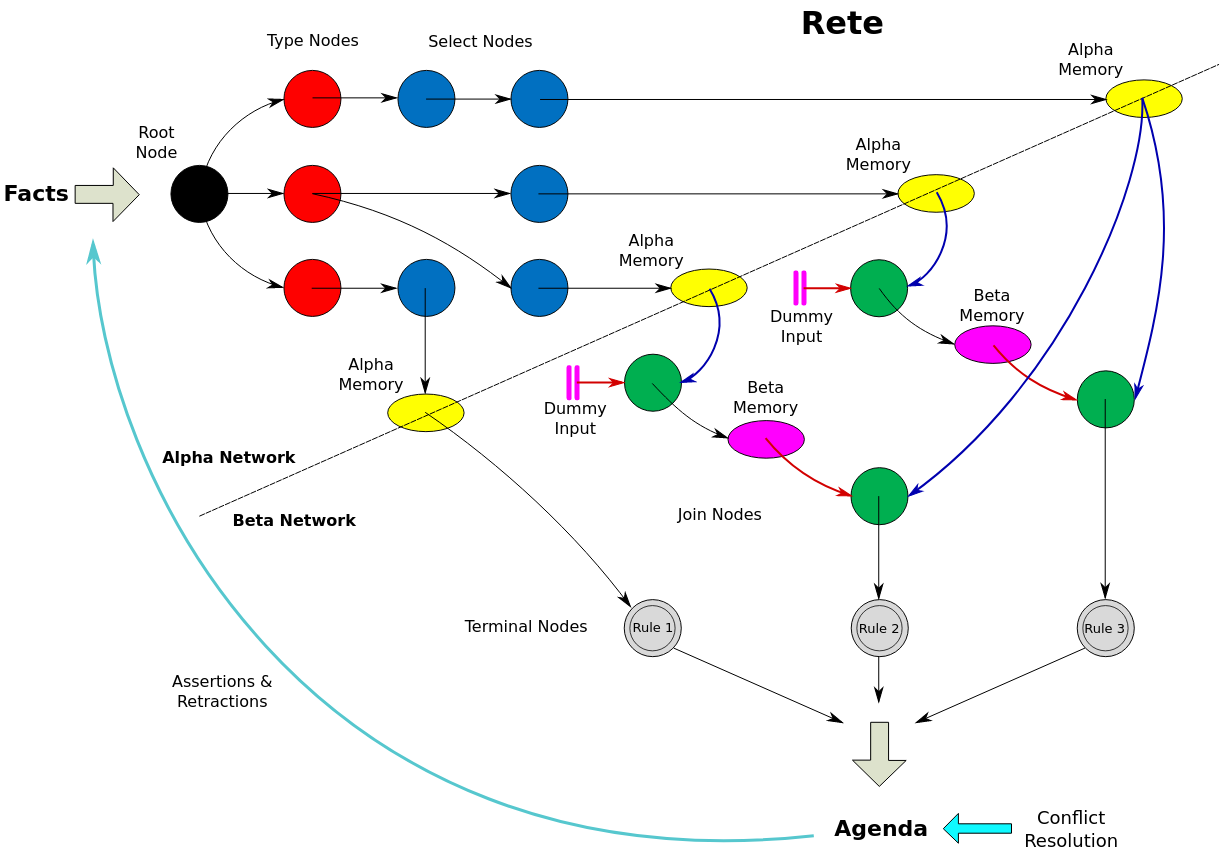
\includegraphics[width=\textwidth]{figures/rete-image.png}
  \caption[Illustrates the basic Rete]{Illustrates the basic Rete\cite{reteimage}}
  \label{fig:rete}
\end{figure}

As said, \acrfull{sec} uses a custom format design particularly for \acrshort{sec} based on regular expressions. We will further examine this rule format under \cref{sub:sec-rule-format}. We will also consider Sigma in greater detail in \cref{sub:sigma} as a possible candidate for replacing the rules used by \acrshort{sec}.

\subsection{SEC rule format}
\label{sub:sec-rule-format}
\acrshort{sec} rule files are simple text-files that contain one or more blocks of key-value pairs. One block is considered one rule. This block contains a set of pre-specified keys that make up how the rule works.

SEC applies each rule sequentially, and will stop looking when it finds a match (unless that specific rule uses the continue keyword). With this knowledge it is possible to optimize the rule set by placing more popular rules nearer the top of the rule set as told by \textcite{rouillard2004real}.

A rule consists of a subset of the following keywords, where some of the keywords are only applicable if some of the keywords holds a special value:
\begin{itemize}
    \item type - which kind of rule
    \item ptype - which type of pattern
    \item pattern - pattern to match event against
    \item desc - rule description
    \item action - action to take if pattern is matched
    \item continue - if set, allows SEC to continue searching for other matching rules
    \item context - boolean statement based on global context variables
    \item thresh - (if applicable) threshold for triggering event
    \item window - (if applicable) time window in seconds
\end{itemize}

for \textbf{type}, there are multiple different possible values:
\begin{itemize}
    \item Single - Match input and execute action.
    \item Suppress - Suppress the matching input which keeps the input from being matched by later rules.
    \item Calendar - Execute action on a given time.
    \item SingleWithSuppress - A combination of Single and Suppress. Match input and execute action, but suppress the matching input for a set period of time afterwards.
    \item Pair - Match input and execute action, then wait until another event arrives and execute second action.
    \item PairWithWindow - Like Pair, but also execute an action if second event does not arrive.
    \item SingleWithThreshold - Count matching input in a time window, if number of matches is above a threshold, execute action and ignore matches for rest of window.
    \item SingleWith2Thresholds - Count matching input in a time window, if number of matches is above a threshold, execute action. Then create new count, and if number of matches drops below the threshold, execute action. 
    \item EventGroup - Count N number of different events and execute action if all of them reach their given threshold.
    \item SingleWithScript - Match value and depending on return-value of external script, do action.
    \item Jump - Submits matching event to another rule set for further processing.
\end{itemize}

For \textbf{ptype}, there are multiple different possible values:

\begin{itemize}
    \item SubStr - pattern is a string that will be searched for in the event
    \item RegExp - pattern is a Perl regular expression
    \item PerlFunc - pattern is a Perl function for matching
    \item Cached - pattern matches previously cached patterns.
    \item TValue - pattern is a boolean value (TRUE/FALSE) that always or never matches.
\end{itemize}

In addition to the above-mentioned values for ptype, they all have (except for TValue) a negated version as well, prefixed with "N" (as in NSubStr, NRegExp, etc).

The following example in figure \cref{sec-example-rule} is a slimmed down version of the "MITRE CAR-2013-04-002: Quick execution of a series of suspicious commands" \cite{CAR2013057:online}. The purpose of the rule is to detect quick execution of commands that a regular user would not frequently do, but that an attacker might run as part of their reconnaissance or exploitation of the system.

As an example, consider that the following events occur within 10 seconds from start to finish:

\begin{enumerate}
    \item \colorbox{blue!30}{Alice ran word.exe on PC1}
    \item \colorbox{green!30}{Bob ran calc.exe on PC2}
    \item \colorbox{red!30}{Mallory ran whoami.exe on PC1}
    \item \colorbox{red!30}{Mallory ran ssh.exe on PC1}
    \item \colorbox{green!30}{Bob ran powershell.exe on PC2}
    \item \colorbox{blue!30}{Alice ran firefox.exe on PC1}
    \item \colorbox{red!30}{Mallory ran powershell.exe on PC1}
    \item \colorbox{red!30}{Mallory ran systeminfo.exe on PC1}
    \item \colorbox{green!30}{Bob ran word.exe on PC2}
    \item \colorbox{blue!30}{Alice ran powerpoint.exe on PC1}
    \item \colorbox{red!30}{Mallory ran hostname.exe on PC1}
\end{enumerate}

If we apply the rule shown in \cref{sec-example-rule}, during the execution, the following events will be created and re-injected into the event stream:

\begin{enumerate}
    \item \colorbox{red!30}{Interesting\_commands\_by\_Mallory\_on\_PC1}
    \item \colorbox{green!30}{Interesting\_commands\_by\_Bob\_on\_PC2}
    \item \colorbox{red!30}{Interesting\_commands\_by\_Mallory\_on\_PC1}
    \item \colorbox{red!30}{Interesting\_commands\_by\_Mallory\_on\_PC1}
\end{enumerate}

These re-injected events will be processed by rule \#4, and when the threshold number of 3 is met for the event "\textit{Interesting\_commands\_by\_Mallory\_on\_PC1}", the rule will trigger its action and write "\textit{Three interesting commands were run on host PC1 by user Mallory}" to the console.

\begin{lstlisting}[
    caption={Example ruleset for detecting quick execution of a series of commands},
    label=sec-example-rule,
    language=Perl]
# Rule 1
type=Single
ptype=RegExp
pattern=(\S+) ran whoami\.exe on (\S+)
desc=$0
action=event Interesting_commands_by_$1_on_$2

# Rule 2
type=Single
ptype=RegExp
pattern=(\S+) ran powershell\.exe on (\S+)
desc=$0
action=event Interesting_commands_by_$1_on_$2

# Rule 3
type=Single
ptype=RegExp
pattern=(\S+) ran hostname\.exe on (\S+)
desc=$0
action=event Interesting_commands_by_$1_on_$2

# Rule 4
type=SingleWithThreshold
ptype=RegExp
pattern=Interesting_commands_by_(\S+)_on_(\S+)
desc=$0
action=write - Three interesting commands were run on host $2 by user $1
window=10
thresh=3
\end{lstlisting}

In addition to the rule show in \cref{sec-example-rule}, we can implement the same rule by using the EventGroup type as show in \cref{sec-example-rule-2}. This rule works similarly as the first rule, but the main difference with EventGroups is that all the event conditions have to be satisfied before the action will trigger. This means that we explicitly have to have all three patterns match, and will not trigger if for instance \textit{whoami.exe} is ran three times in a row.

\begin{lstlisting}[
    caption={Example ruleset 2 for detecting quick execution of a series of commands},
    label=sec-example-rule-2,
    language=Perl]
type=EventGroup3
ptype=RegExp
pattern=(\S+) ran whoami\.exe on (\S+)
ptype2=RegExp
pattern2=(\S+) ran powershell\.exe on (\S+)
ptype3=RegExp
pattern3=(\S+) ran hostname\.exe on (\S+)
desc=Three interesting commands were run on host $2 by user $1
actiom=write - Three interesting commands were run on host $2 by user $1
window=10
\end{lstlisting}

This is not an extensive listing of the features in the \acrshort{sec} rule language, but covers what is needed for the rest of the thesis. For a deeper dive into \acrshort{sec} rules with more examples, the reader is referred to the paper \citetitle{rouillard2004real} by \textcite{rouillard2004real} and the \acrshort{sec} man-pages \cite{secman}.

\subsection{Sigma}
\label{sub:sigma}
\url{https://github.com/Neo23x0/sigma}

Sigma is an open standard for rules that are used to generically describe searches in log data. It is primarily used as a high-level rule that transcompile into SIEM queries like Splunk, ElasticSearch, QRadar, etc. The rules are written in YAML (Yet Another Markup Language), and are key-value based.
\\
The following example Sigma rule is a basic rule that detects running \lstinline{ipconfig}, \lstinline{arp} and \lstinline{echo} within a ten second timeframe, filtered by the \lstinline{MachineName} key in the event: \todo{We should add some examples of what an event actually looks like, to make it more obvious to the reader what we are talking about here}

\begin{lstlisting}[
    basicstyle=\small
]
title: Quick Execution of a Series of Suspicious Commands
id: 61ab5496-748e-4818-a92f-de78e20fe7aa
description: Detects multiple suspicious process in a limited timeframe
status: experimental
references:
    - https://car.mitre.org/wiki/CAR-2013-04-002
author: Martin Ingesen
modified: 2020/01/01
tags:
    - car.2013-04-002
logsource:
    category: process_creation
    product: windows
detection:
    selection:
        CommandLine:
            - ipconfig
            - arp
            - echo
    timeframe: 10s
    condition: selection | count() by MachineName > 3
falsepositives:
    - False positives depend on scripts and
    administrative tools used in the monitored environment
level: low
\end{lstlisting}
The format contains some required and some optional fields, and is extensible with our own custom fields.

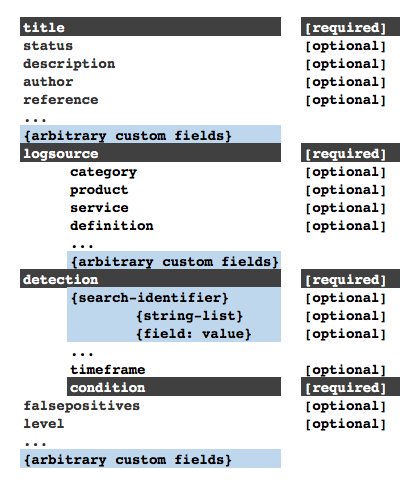
\includegraphics[scale=0.525]{figures/new-rule-format/Sigma_Schema.png}

Image source: \url{https://github.com/Neo23x0/sigma/wiki/Specification}

